%!TeX program = xelatex
\documentclass[11pt]{article}

\usepackage{graphicx}
\usepackage{fancyhdr}
\usepackage{geometry}
\usepackage[utf8]{inputenc}
\usepackage{enumitem}
\usepackage{amsmath} 
\usepackage{multirow}
\usepackage{caption}
\usepackage{float}
\usepackage{fontspec}
\usepackage{cite}
\usepackage{listings}
%\setmainfont{UT Sans}
\usepackage{geometry}
\usepackage{xcolor}

\lstdefinestyle{customc}{
	belowcaptionskip=1\baselineskip,
	breaklines=true,
	frame=L,
	xleftmargin=\parindent,
	language=C,
	showstringspaces=false,
	basicstyle=\large\ttfamily,
	keywordstyle=\bfseries\color{green!40!black},
	commentstyle=\itshape\color{purple!40!black},
	identifierstyle=\color{blue},
	stringstyle=\color{orange},
}

\lstset{escapechar=@,style=customc}

\geometry{a4paper,left=20mm,right=20mm,total={160mm,220mm}}
\pagestyle{fancy}
\thispagestyle{plain}
\fancyheadoffset{0cm}
\rhead{\textit{Andrei Vasilcoi}\\Grupa 4452}

\renewcommand*\contentsname{Cuprins}
\renewcommand*\tablename{Tab.}
\renewcommand*\figurename{Fig.}
\renewcommand\refname{Bibliografie}
\renewcommand{\theenumi}{\Alph{enumi}}
\author{Andrei Vasilcoi}
\newcommand{\EqRow}{\vspace{1.5mm}}
\begin{document}
\begin{titlepage}

\newcommand{\HRule}{\rule{\linewidth}{0.5mm}}
	
\begin{center}
	%autor si indrumator mai jos
\textsc{\LARGE Universitatea Transilvania din Brașov}\\[0.5cm]

\includegraphics[width=0.25\textwidth]{logo_ut.jpg}\\[0.5cm]
\textsc{\Large Facultatea de Inginerie Electrică și Știința Calculatoarelor}\\[0.5cm]
\textsc{\large Departament Automatică și Informatică Aplicată}\\[1.5cm]
\HRule\\[0.5cm]
{\Large Proiect \textit{Acționare electrică reglabilă reversibilă cu convertor fără curenți de circulație}}\\[0.5cm]
\HRule\\[2.5cm]
\begin{minipage}{1\textwidth}
	\begin{flushleft}
		\large
		\textit{Autor}\\
		Andrei \textsc{Vasilcoi}\\
	\end{flushleft}
\end{minipage}
~
\end{center}
\centering
\vspace{5cm}
{\large Decembrie 2018, Brașov}\\[5cm]
\end{titlepage}

\newpage
\pagenumbering{arabic}
\tableofcontents

\newpage	
\section{Tema proiectului}

Sa se proiecte o actionare electrica reglabila reversibila cu convertor fara curenti de circulatie. Proiectul va cuprinde: 
\begin{enumerate}[label=$\bullet$]
	\item calculul circuitului de reglare al curentului; 
	\item calculul circuitului de reglare al turatiei. 
\end{enumerate}
Se va folosi un motor de c.c. cu excitalie independenta comandat pe indus, utilizand ca element de executie o punte cu tiristoare complet comandata.

\begin{center}
\captionof{table}{Date de proiectare}
\begin{tabular}{|c|c|c|c|c|c|c|c|c|c|c|}
	\hline
	P & $U_N$ & $\eta$ & n & ${GD_r}^2$ & ${GD_s}^2$ & $\Delta$n&$\sigma$&$\epsilon_{st}$ & $I_{lim}/I_n$&Precizia
	\\
	\hline
	3.7&190&0.77&2500&0.13&0.07&190-2500&6&0&1.5&5
	\\
	\hline
\end{tabular}
\end{center}

\newpage
\section{Generalitati}

Motoarele de curent continuu se utilizeaza frecvent in actionariie electrice reglabile datorita proprietatilor lor favorabile (reglare fina si in limite largi a turatiei.). Dezavantajul principal al acestor motoare il constituie prezenta colectorului, care limiteaza superior puterea si turatia si mareste momentul de inertie. 

In figura 1.a este reprezentata principal o masina de curent continuu cu doi poli avand statorul 5 si indusul cilindric A. Indusul si polii sunt confectionati din tole pentru a micsora pierderile in fier. La masinile de puteri mari si cu calitati dinamice superioare se confectioneaza si restul statorului din tole. Polii principali P sunt prevazuti cu infasurarea de excitatie, parcursa de curentul de excitatie Ie , care produce fluxul magnetic principal Φe. Acest flux se inchide prin rotor (indus) si stator. In crestaturile indusului este plasata infasurarea indusului care, prin intermediul colectorului si a periilor p, este alimentata (in functionarea ca motor) de la retea cu curentul Ia. 

Conductoarele indusului sunt repartizate uniform de-a lungul intregii circumferinte a indusului si rezulta o repartizare uniform de-a lungul intregii circumferinte a indusului si rezulta o repartizare a curentului dupa cum se indica in figura 1.a. O asemenea repartizare produce un camp de reactie a indusului a carui axa este perpendiculara pe axa campului inductor principal. 

Fluxul de reactie transversal corespunzator Φa este, datorita intrefierului mare in directia transversala, mult mai mic decat fluxul de excitatie Φe. Infaurarea de compensatie C, plasata in piesele polare si parcursa de curentul prin indus Ie, reduce si mai mult fluxul in directia transversala. In general numai masinile mari sunt prevazute cu infasurari de compensatie. 
Campul magnetic inzona de comutatie este influentat de polii auxiliari PA, excitati de curentul prin indus, pentru a se atinge o comutatie fara scantei.

\begin{figure}[H]
	\centering
	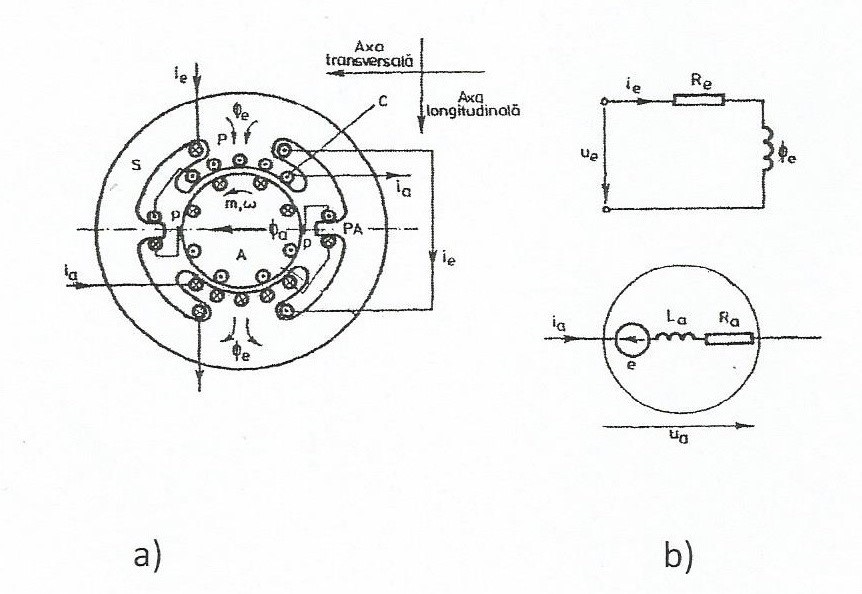
\includegraphics[width=.7\linewidth]{fig1.jpg}
	\captionof{figure}{Masina de curent continuu, cu excitatie separata}
	\label{fig:test2}
\end{figure}

Actiunea inductiva a indusului poate fi reprezentata printr-o inductivitate concentrata La. Deoarece infasurarea de compensatie si infasurarea polilor auxiliari se gasesc de asemenea in axa periilor (transversala) actiunea lor se posta lua in considerare prin La.

\section{Motorul de curent continuu cu excitatie separata \\
	Ecuatii diferentiale si schema bloc}
Schema echivalenta a motorului de curent continuu cu excitatie separata (independenta), care a fost deja reprezentata in figura 1.b, se modifica in sensul ca parametrii concentrati Ra si La se reprezinta in afara indusului (figura 2)
\begin{figure}[H]
	\centering
	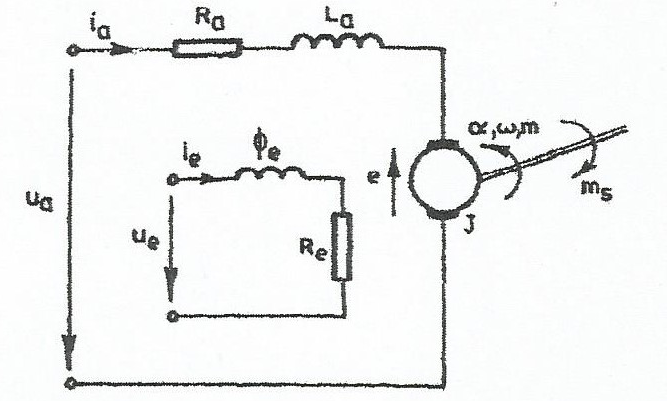
\includegraphics[width=.5\linewidth]{fig2.png}
	\captionof{figure}{Schema echivalenta a motorului de curent continuu cu excitatie separata}
	\label{fig:test2}
\end{figure}

Ca marimi de intrare actioneaza tensiunea aplicata indusului ua, tensiunea aplicata circuitului de excitatie ue si cuplul de sarcina ms.Φe este fluxul de excitatie, m este cuplul electromagnetic al motorului , iar J momentul de inertie a maselor cu miscare de rotatie. 
Aplicand teorema a doua a lui Kirchhoff circuitului indusului rezulta:
\begin{align}
u_a=e+R_ii_a+L_a\frac{di_a}{dt}
\end{align}
unde s-a neglijat caderea de tensiune la periile masinii, care depinde neliniar de curentul prin indus.

In acelasi mod, pentru circuitul de excitatie se obtine:
\begin{align}
u_e=R_ei_e+\frac{d\Phi_e}{dt}
\end{align}
Tensiunea electromotoare indusa prin rotatie va fi:
\begin{align}
e=k\Phi_e\omega, cu\ k = \frac{pN}{2\pi a}
\end{align}
unde:
\begin{enumerate}[label=$\bullet$]
	\item N - numarul de conductoare activa a infasurarii indusului;
	\item p - numarul de perechi de poli; 
	\item a - numarul de perechi de cai de curent ale infasurarii indusului;
	\item $\omega$ - viteza unghiulara a indusului (rotorului)  
\end{enumerate}
Cuplul electromagnetic exercitat asupra rotorului motorului este:
\begin{align}
m=k\Phi_ei_a
\end{align}
Ecuatia de miscare se poate scrie sub forma:
\begin{align}
m-m_s=J\frac{d\omega}{dt}
\end{align}
Ecuatia vitezei unghiulare este:
\begin{align}
\omega=\frac{d\alpha}{dt}
\end{align}
Ecuatia (1) se poate pune sub forma:
\begin{align}
T_a\frac{di_a}{dt}+i_a=\frac{1}{R_a}(u_a-e)
\end{align}
Unde $T_a=L_a/R_a$  este constanta de timp a circuitului indusului.
Ecuatia (2) scrisa sub forma:
\begin{align}
\frac{d\Phi_e}{dt}=u_e-R_ei_e
\end{align}
reprezinta ecuatia diferentiala a unui element de integrare (integrator).
\begin{figure}[H]
	\centering
	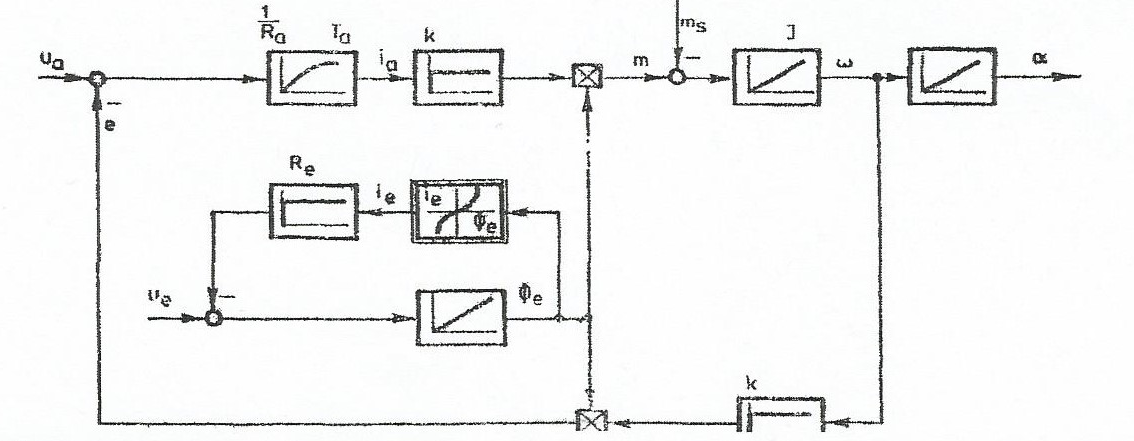
\includegraphics[width=.8\linewidth]{fig4.png}
	\captionof{figure}{Schema bloc a motorului de curent continuu cu excitatie separata (marimi absolute).}
	\label{fig:test2}
\end{figure}
Ecuatiile (7), (8), (3), (4), (6) descriu comportarea dinamica a motorului de curent continuu cu excitatie separata. Schema structu ru la sa u sche ma bloc corespunzatoare acestor ecuatii diferentialee cuplate este ilustrata in Fig. 3.

Marimile variabile care apar in schema bloc din figura 3 au diferite dimensiuni. Pastrarea neschimbata a acestor marimi ar complica calculul prin relatii dimensionale complicate. Din aceasta cauza se obisnuieste ca toate marimile sa se raporteze, adica sa devina marimi adimensionale. Se ajunge astfel la sistem de unitati relative care usureaza calculele, in special cele efectuate pe calculator.
\begin{figure}[H]
	\centering
	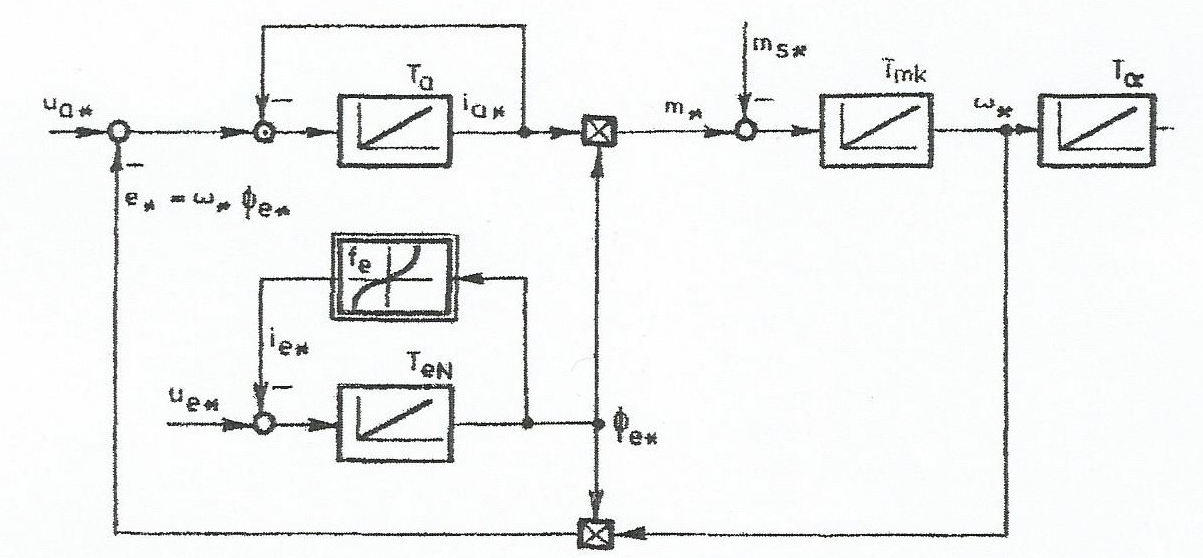
\includegraphics[width=.8\linewidth]{fig5.png}
	\captionof{figure}{Schema bloc a motorului de curent continuu cu excitatie separata (marimi relative)}
	\label{fig:test2}
\end{figure}
\section{Caracteristici mecanice stationare la comanda pe indus}
La comanda pe indus fluxul de excitatie se mentine constant, la valoarea nominala $\Phi_e=\Phi_{eN}$ si se modifica tensiunea de alimentare $u_a$;

Pentru $\Phi_e=\Phi_{eN}\frac{\Phi_{e}}{\Phi_{en}}$ dispar astfel ambele semne de multiplicare din schema bloc.
\begin{center}
	$\omega*=u_{a^*}-m_{s^*}$\\
	$i_{a^*}=m_{s^*}$
\end{center}
Caracteristicile mecanice $W* (m_{s^*})$ reprezinta o familie de drepte, parelele cu 
caracteriastica mecanica naturala $u_{a^*}=\frac{U_{aN}}{U_a}=1$ avand drept parametru $u_{a^*}=\frac{U_{aN}}{U_a}$

Caracteristicile sunt valabile in toate cele patru cadrane, deci exista posibilitatea unei reversari continue a turatiei si cuplului. Caracteristicile mecanice obtinute prin variatia tensiunii de alimentare se numesc carecteristici mecanice artificiale de tensiune. Deoarece tensiunea aplicata indusului u, este raportata la valoarea sa nominala, ne intereseaza numai domeniul $-1 \leq \frac{u_a}{u_{aN}} \leq 1$; la depasirea importanta a acestui domeniu se inrautateste 
comutatia (apar mai intai scantei la perii si apoi, posibil, foc la colector). 

Curentul prin indus (figura 5.b) este proportional cu cuplul, iar tensiunea indusului nu are nici o influenta. Cuplul este raportat la cuplul de pornire pe caracteristica mecanica naturala $m_a$ (la motoarele mari $m_a = (8 ... 10)mN)$. De aceea domeniul de functionare normal este $-0.2 \leq \frac{m}{m_0}\leq 0.2$.
\begin{figure}[H]
	\centering
	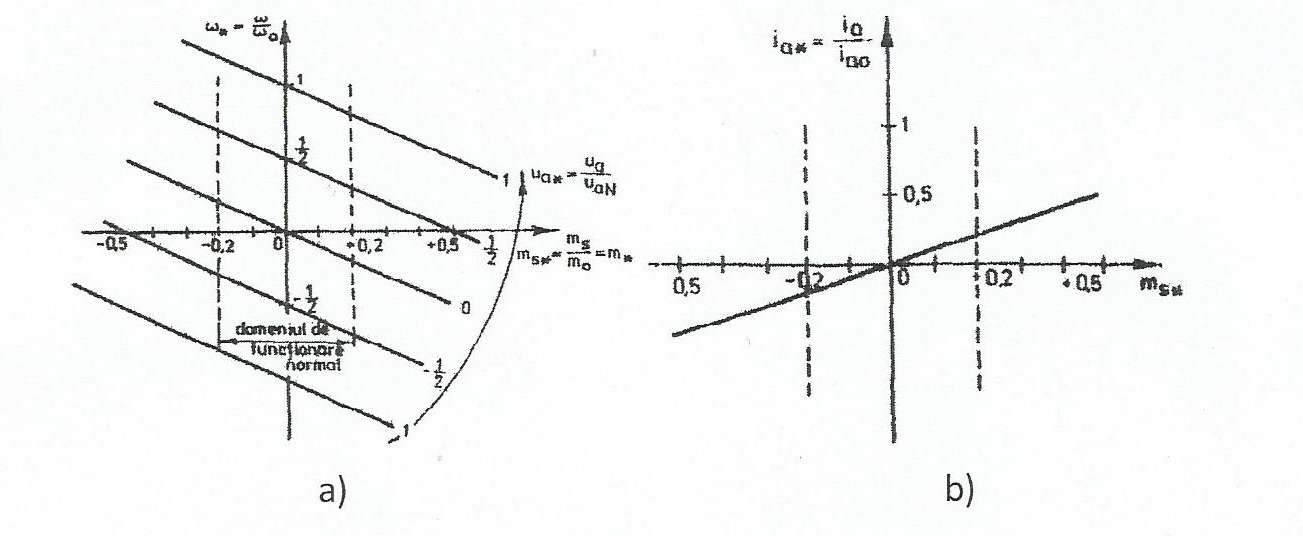
\includegraphics[width=.8\linewidth]{fig6.png}
	\captionof{figure}{Comanda pe indus a) caracteristici mecanice artificiale de tensiune b) caracteristica $i_{a^*}(m_{s^*})$}
	\label{fig:test2}
\end{figure}
In afara acestui domeniu, datorita reactiei indusului $\Phi_{e}(I_a)$, caracteristicile mecanice prezentate sunt numai partial valabile; de asemenea apar probleme de comutatie. 

Deoarece cuplul electromagnetic m respectiv cuplul de sarcina ma este raportat la valoarea cuplului de pornire, pe caracteristica mecanica naturala mo caracteristicile mecanice stationare la comanda pe indus (figura 5.a) apar mai inclinate decat cele reprezentate in marimi absolute si intalnite frecvent in lucrari de specialitate.

La flux de excitatie constant $\Phi_{e}=\Phi_{eN}$ modificarea tensiunii indusului produce o deplasare paralela a caracteristicilor mecanice in timp ce caracteristica curent-cuplu ramane constanta. Acest lucru apare deosebit de avantajos la actionarile electrice regla bile, deoarece parametrii circuitului de reglare ramain neschimbati; avem de-a face cu un element liniar. 
\section{Reglarea turatiei motoarelor de curent continuu}
In practica, alegerea unei actionari de curent continuu este determinata in mod obisnuit de posibilitatea obtinerii unui domeniu larg de variatie a turatiei, domeniu impus de procesul tehnologic. Pentru a se obtine insa comportarea de functionare dorita, la perturbatii ale retelei. de alimentare si ale sarcinii mecanice, actionarea trebuie sa fie automatizata. 

Pe de alta parte, indusul motoarelor mari prezinta o rezistenta mica si in momentul pornirii la tensiunea nominala rezulta prin indus un curent foarte mare. In functionarea stationara nu se intalneste asemenea situatie, deoarece curentul este determinat de diferenta dintre tensiunea aplicata indusului si. tensiunea electromotoare indusa. In regim nestationar este posibil ca, datorita unei schimbari prea rapide a tensiunii sau turatiei, sa apara un curent nepermis de mare. De aceea, pentru protejarea motorului, a sursei de alimentare, si a sarcinii mecanice se prevede o limitare rapida a curentului prin indus si deci a cuplului electromagnetic dezvoltat de motor.
\begin{figure}[H]
	\centering
	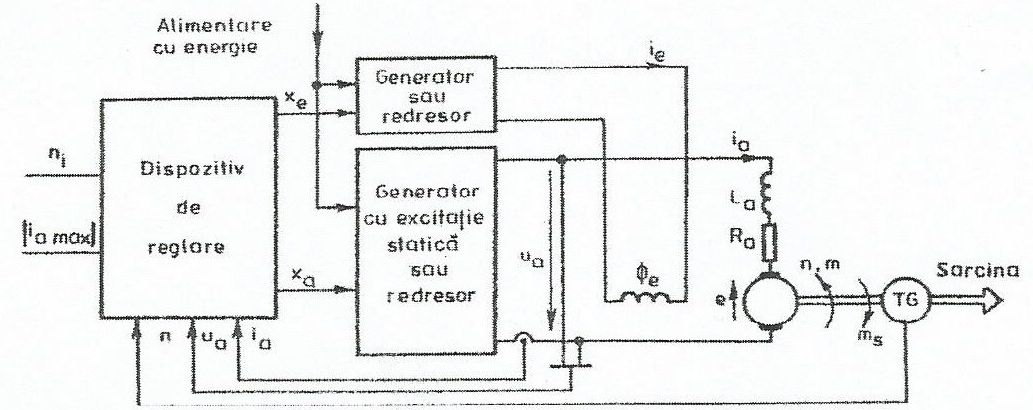
\includegraphics[width=.8\linewidth]{fig7.png}
	\captionof{figure}{Schema de principiu a unei actionari de curent continuu reglabile}
	\label{fig:test2}
\end{figure}
\section{Reglarea turatiei prin comanda pe indus}
Pentru a se micsora supracurentul prin indus si pentru a proteja motorul, fluxul de excitatie trebuie mentinut la valoarea nominala. 

In figura 7 s-a reprezentat circuitul indusului motorului si sursa de alimentare a indusului (elementul de executie). S-a notat cu ea tensiunea sursei de alimentare a indusului, comandata prin. xa, tensiune care, datorita impedantei interne (R, LJ, nu corespunde cu tensiunea u, aplicata la bornele motorului. Impedanta interna a elementului de executie trebuie luata de asemenea in considerare la definirea marimilor de referinta.
\begin{figure}[H]
	\centering
	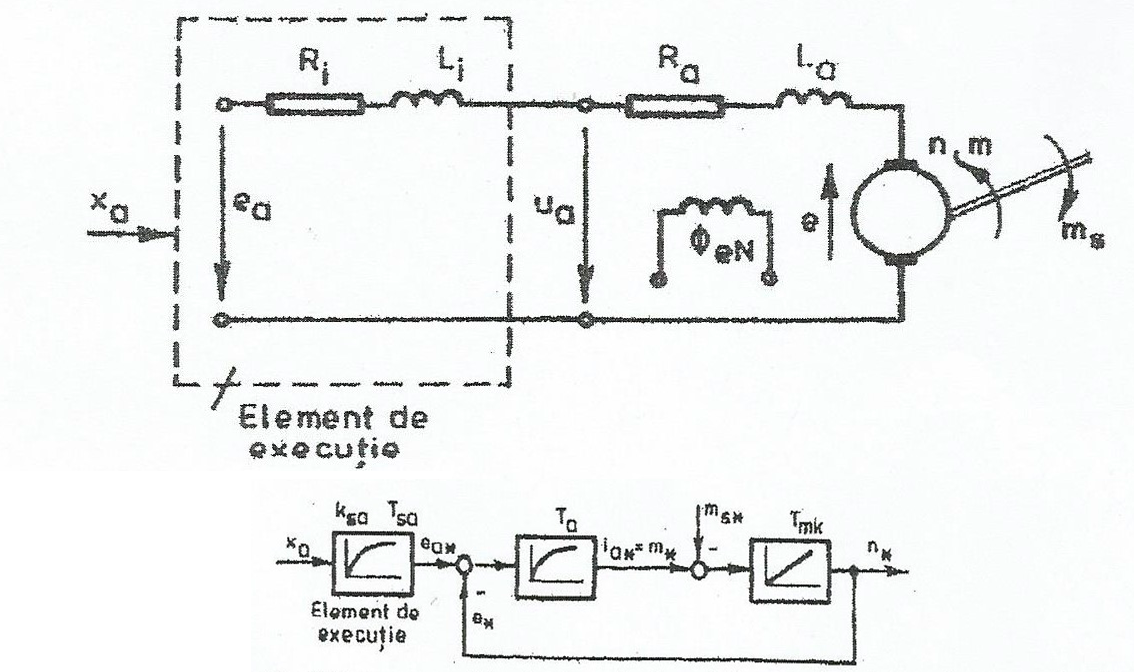
\includegraphics[width=.8\linewidth]{fig8_fin.png}
	\captionof{figure}{Schema echivalenta a indusului motorului si a elementului de executie}
	\label{fig:test2}
\end{figure}
\begin{center}
	$i_a=\frac{u_{aN}}{R_a+R_i}$ \ 	$T_a=\frac{L_a+L_i}{R_a+R_i}$
\end{center}
\begin{figure}[H]
	\centering
	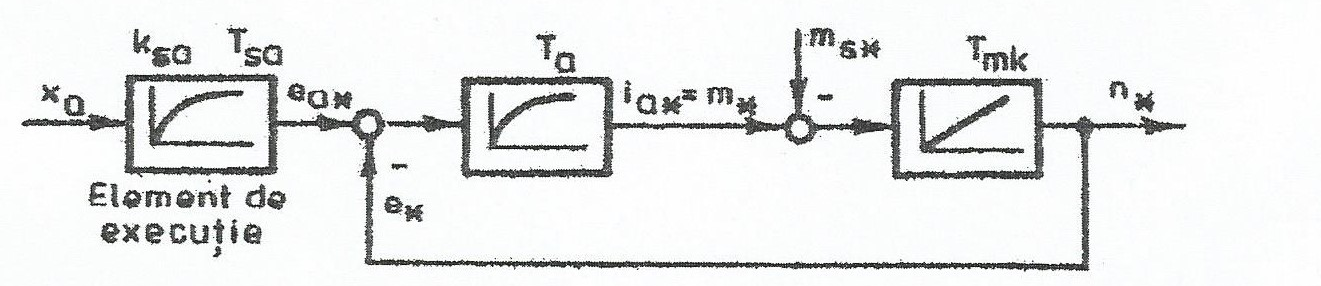
\includegraphics[width=.8\linewidth]{fig9.png}
	\captionof{figure}{Schema bloc a sistemului motor de curent continuu cu excitatie separata}
	\label{fig:test2}
\end{figure}
Pentru sursa de tensiune comandata a indusului s-a considerat un element inertial de ordinul intai (cu amplificarea ksa si constanta de timp TsJ. Valoarea constantei de timp Tsa la un redresor comandat are valoarea de (1. .. 5)ms. Constanta de timp a indusului Ta are inmod obisnuit valori cuprinse intre 10 si 100 ms; ea este determinata de impedanta circuitului indusului considerand o eventuala bobina de netezire, care la alimentarea de la redresoare este necesara pentru micsorarea ondulatiei curentului. 

Constanta, de timp Tmk se refera la momentul de inertie total al actionarii raportat la arborele motorului; ea poate varia de la ordinul milisecundelor la cateva secunde. 

Pentru reglarea turatiei cu limitarea curentului prin indus, cel mai potrivit principiu de reglare este procedeul reglarii in cascada. Reglarea in cascada are cateva insusiri importante: 
\begin{enumerate}[label=$\bullet$]
	\item permite, pe langa reglarea marimii principale (in cazul de fata turatia), limitarea marimilor auxiliare (de exemplu curentul prin indus); 
	\item fractioneaza functia de transfer a elementului de executie si procesului in portiuni, astfel incat fiecarui regulator i se repartizeaza una sau cel mult doua constante de timp importante, ceea ce face ca optimizarea se se poata realiza un regulator PID sau cu variante mai simple ale acestuia; 
	\item permite o simetrizare a operatiilor de acordare optimala a regulatoarelor 
\end{enumerate}
Pentru schema bloc a motorului se pot scrie ecuatiile:
\begin{align}
T_a\frac{di_{a^*}}{dt}+i_{a^*}=e_{a^*}-e_*
\end{align}
\begin{align}
e_*=n_*
\end{align}
\begin{align}
T_{mk}\frac{dn_{*}}{dt}=m_{*}-m_{s^*}
\end{align}
\begin{align}
i_{a^*}=m_*
\end{align}
Pe baza ecuatii lor de mai sus cu notatiile: Ea(s) = L{ea*}; N(s) = L{n*} rezulta schema bloc a motorului reprezentata in figura 9.
\newpage

\nocite{*}
\bibliographystyle{ieeetr}
\bibliography{bibliografie}

\end{document}